\documentclass{beamer}
\usepackage{verbatim}
\usetheme{Boadilla}
\title{CMBFAST}
\author{Floor Terra}
%\date{}

\begin{document}
	\begin{frame}
		\titlepage
	\end{frame} 
	
	\begin{frame}
		\frametitle{The big bang}
		\framesubtitle{A simple model}
		\begin{itemize}
			\item The universe starts small, hot and dense
			\item The universe expands and cools
			\item Recombination ($z=1100$, $T=4000K$)
			\item Surface of last scattering
			\item Universe expands while photons travel freely
			\item CMB is measured by Arno Penzias and Robert Woodrow Wilson ($z=1$, $T=2.725K$)
		\end{itemize}
	\end{frame}
	
	\begin{frame}
		\frametitle{WMAP}
		\framesubtitle{What do we see today?}
		\begin{center}
			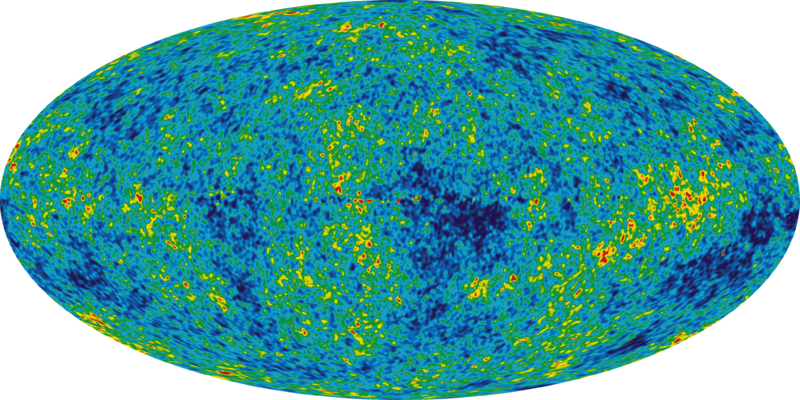
\includegraphics[width=90mm]{WMAP.png}
		\end{center}
	\end{frame}
	
	\begin{frame}
		\frametitle{WMAP}
		\framesubtitle{The data}
		\begin{itemize}
			\item Mean temperature $T=2.725K$
			\item Variations of XXX
			
		\end{itemize}
	\end{frame}
	
	\begin{frame}
		\frametitle{The CMBFAST code}
		\framesubtitle{A line-of-sight integration approach to cosmic microwave background anisotropies}
		\begin{itemize}
			\item Written by Uros Seljak and Matias Zaldarriaga.
			\item Article published in 1996
			\item The first fast CMB code
			\item Written in the FORTRAN programming language
		\end{itemize}
	\end{frame}
	
	\begin{frame}
		\frametitle{The problems with CMBFAST}
		\framesubtitle{FORTRAN}
		\begin{center}
			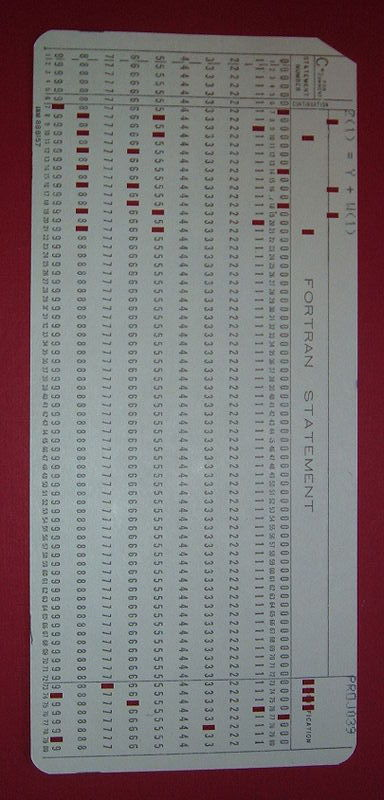
\includegraphics[width=90mm]{punch_card.jpg}
		\end{center}
	\end{frame}
	
	\begin{frame}
		\frametitle{The problems with CMBFAST}
		\framesubtitle{Interactive}
		\begin{itemize}
			\item CMBFAST is designed for interactive use
			\item This makes it hard to automate
				\begin{itemize}
					\item Parameter fitting
					\item batch processing
					\item Play with the code (educational use)
				\end{itemize}
		\end{itemize}
	\end{frame}
	
	\begin{frame}
		\frametitle{py-cmbfast}
		\framesubtitle{A python wrapper around the CMBFAST code}
		\begin{itemize}
			\item Suited for both interactive and scripted use
			\item Easy to use
				\begin{center}
					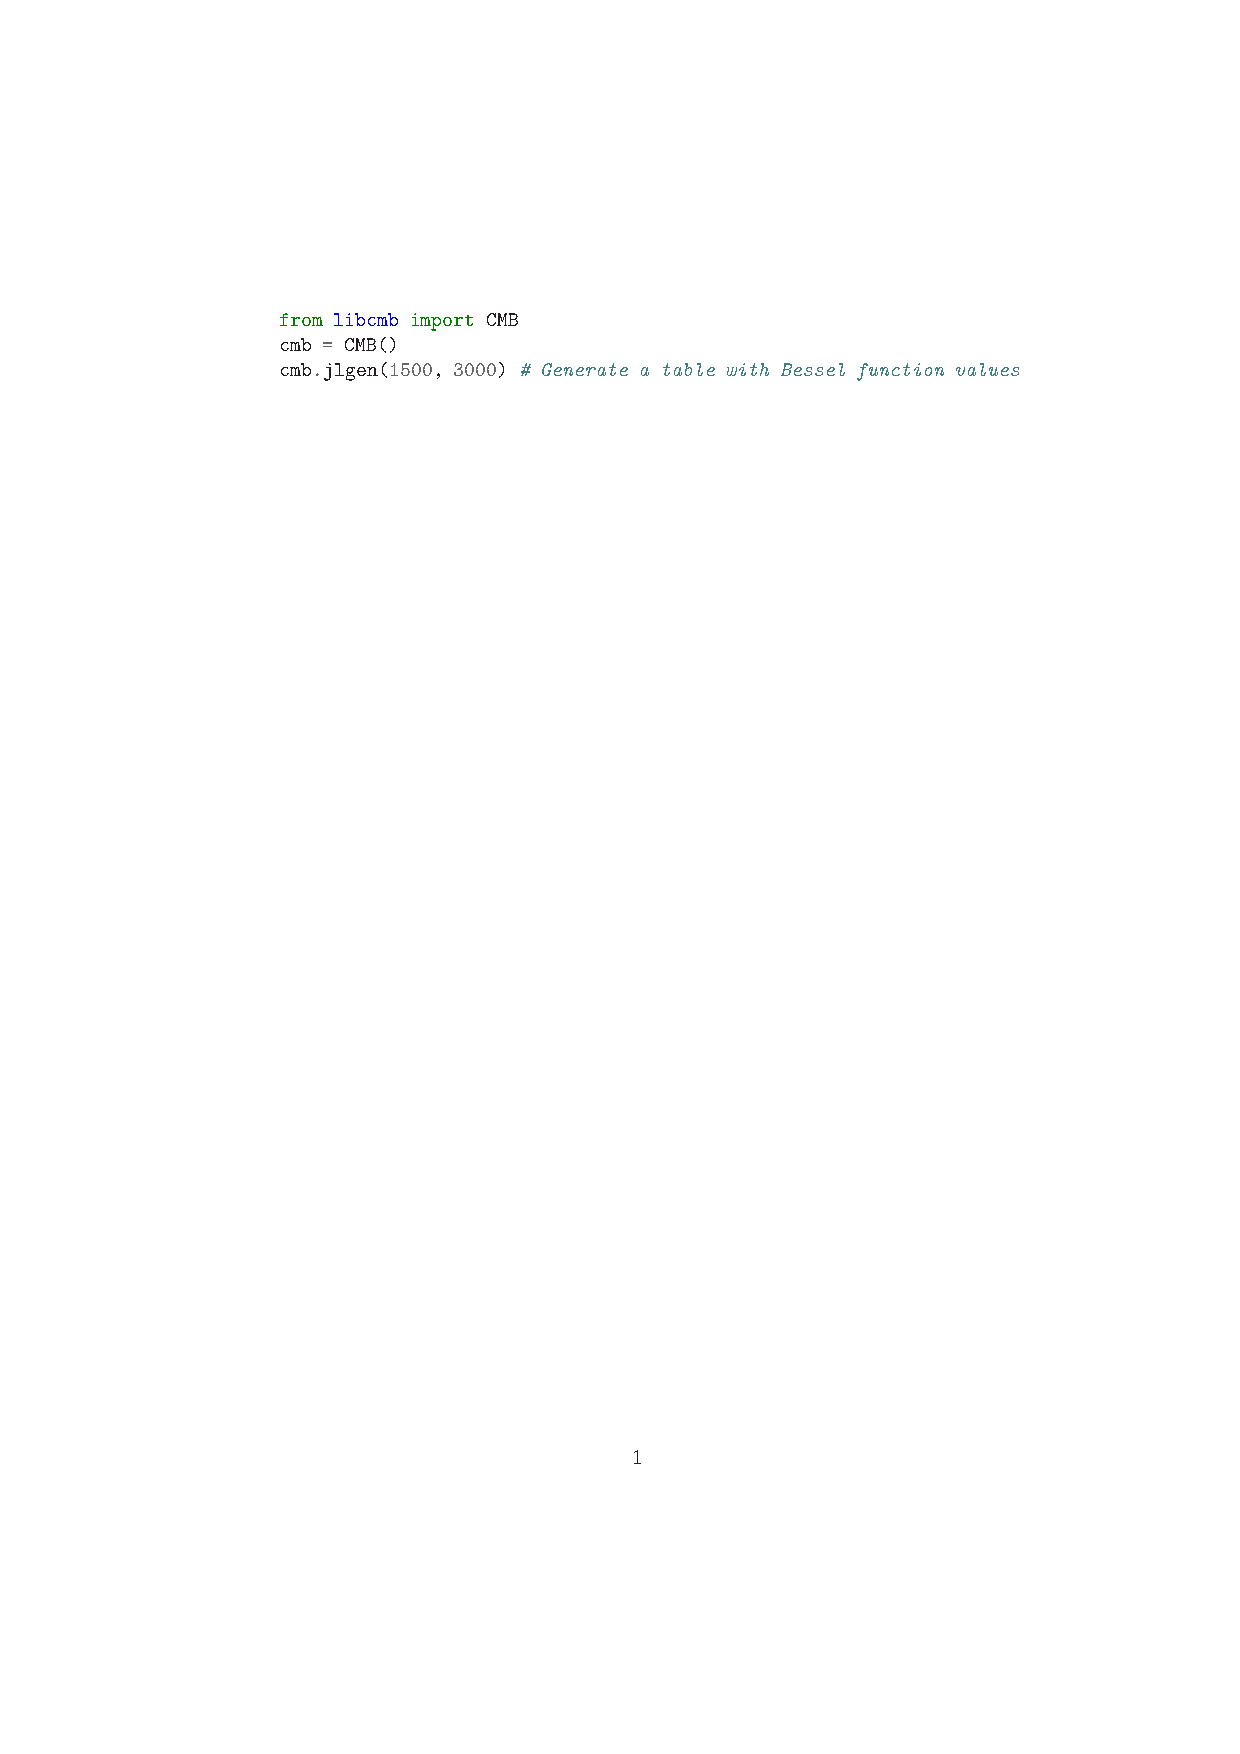
\includegraphics{sample.pdf}
				\end{center}
		\end{itemize}
	\end{frame}

\end{document}
